\documentclass{article}

\usepackage{arxiv}

\usepackage[utf8]{inputenc} % allow utf-8 input
\usepackage[T1]{fontenc}    % use 8-bit T1 fonts
\usepackage{hyperref}       % hyperlinks
\usepackage{url}            % simple URL typesetting
\usepackage{booktabs}       % professional-quality tables
\usepackage{amsfonts}       % blackboard math symbols
\usepackage{nicefrac}       % compact symbols for 1/2, etc.
\usepackage{microtype}      % microtypography
\usepackage{lipsum}		% Can be removed after putting your text content
\usepackage{amssymb,amsmath,amsthm}
\usepackage{listings}
\usepackage{graphicx}
\usepackage{subfig}
\usepackage{apacite}
\usepackage{algorithm}
\usepackage{algorithmicx}
\usepackage{algpseudocode}
\usepackage{kbordermatrix}% http://www.hss.caltech.edu/~kcb/TeX/kbordermatrix.sty
\usepackage{todonotes}

\newtheorem{theorem}{Theorem}
\DeclareMathOperator\supp{supp}

\title{Sampling from the Bayesian poster of an agent-based model given partial observations}

%\date{September 9, 1985}	% Here you can change the date presented in the paper title
%\date{} 					% Or removing it

\author{
  Daniel Tang\\
    Leeds Institute for Data Analytics, University of Leeds, UK\thanks{This project has received funding from the European Research Council (ERC) under the European Union’s Horizon 2020 research and innovation programme (grant agreement No. 757455)}\\
  \texttt{D.Tang@leeds.ac.uk}\\
  \AND
  Nick Malleson\\
  School of Geography, University of Leeds, UK\\  
  %% examples of more authors
  %% \AND
  %% Coauthor \\
  %% Affiliation \\
  %% Address \\
}


\begin{document}
\maketitle

\begin{abstract}
The discipline of data assimilation (DA), sometimes known as data fusion, addresses the problem of how to make use of noisy, imcomplete experimental observations to provide information about unobserved properties of a dynamical system. DA has developed rapidly in some areas of research, notably weather forecasting, but relatively little progress has been made in DA techniques applicable to agent based modelling. Agent Based Models (ABMs) consist of `agents' which often make discrete choices from a number of possible actions, meaning the space of model trajectories is not continuous and we cannot use techniques based on gradient ascent, such as 4D-VAR, that require the gradient of the posterior in this space. In addition, a set of observations will typically refute the vast majority of model trajectories, making it difficult to even identify trajectories that could have given rise to the observations, and so making it challenging to use algorithms that rely on perturbing the current solution such as non-gradient optimisation or most sampling algorithms.

Here we present an algorithm that generates samples of the time evolution of an agent based model, given a set of noisy, incomplete experimental observations of the system. The algorithm approximates the set of possible trajectories as a linear program and uses an extension of the simplex algorithm to provide a proposal function for Markov-Chain-Monte-Carlo sampling.

We demonstrate the algorithm by performing data assimilation in an agent-based, spatial predator-prey model.
\end{abstract}

% keywords can be removed
\keywords{Data assimilation, Bayesian inference, Agent based model, Integer linear programming, predator prey model}

\section{Introduction}

Agent-based modelling (ABM) has become a popular tool for use in modelling the interactions of many discrete, heterogeneous entities, such as humans or animals. In such applications we often have noisy, aggregated and/or incomplete observations of the agents over some period of time and would like to use our ABM to model what happened to the agents during this time period, given our observations. However, this is not straightforward as we don't know the complete start-state of the model, or the exact behavioural decisions the agents would need to make in order to reproduce our observations, so simply running the model forward is not an option. The problem is better framed in terms of probabilistic inference: given the model, our prior beliefs about the start state and our observations, what is the probability distribution over all possible histories over the observed period? This is the problem of Data assimilation (DA) and the subject of this paper. Note that this problem is distinct from the problem of model estimation or parameter optimisation~\cite{thiele_facilitating_2014} which we do not address here.

This paper presents a new method that will allow for \textit{data assimilation} (DA) to be applied to ABMs in order to make inference about the evolution of the agents over an observed time priod. DA has developed rapidly in applications such as weather forecasting~\cite{kalnay_atmospheric_2003} and the earth sciences more broadly~\cite{reichle_data_2008}, but little progress has been made in developing techniques that are applicable when the dynamical system is an agent based model. Many DA methods rely on the differentiability of the posterior distribution~\cite{lewis_dynamic_2006}, but since ABMs consist of `agents' that often make discrete choices from a number of possible actions, the space of model trajectories is not continuous and techniques based on gradient ascent, such as 4D-VAR~\cite{talagrand_assimilation_1997} cannot be used. 
In addition, the majority of model trajectories will be refuted by the observations, making it challenging to use algorithms that rely on perturbing the current solution such as non-gradient optimisation or most sampling algorithms. Some studies have tried to apply well-known DA methods such as Particle Filters and variants of the Kalman Filter to ABMs in applications such as crime~\cite{lloyd_exploring_2016}, bus routes~\cite{kieu_dealing_2020}, pedestrian dynamics~\cite{wang_data_2015, ward_dynamic_2016, clay_realtime_2020, malleson_simulating_2020} and population movement~\cite{lueck_who_2019}, but these have not scaled well and the lack of DA techniques for ABM remains a serious methodological limitation. Other existing techniques for sampling from discrete probability distributions include discrete hit-and-run~\cite{baumert2009discrete} but because of the extreme sparsity of feasible points in the space of ABM trajectories this is unlikely to be efficient. Universal hashing~\cite{meel2016constrained} provides a promising alternative, but in our experience this doesn't scale to the number of dimensions needed for our application. 

Here we present an algorithm that generates samples of the time evolution of an agent based model given a set of noisy, incomplete experimental observations of the system. The algorithm approximates the set of possible trajectories as a linear program and adapts techniques used in linear programming to provide a proposal function for Metropolis-Hastings sampling. We demonstrate the algorithm by performing data assimilation in an agent-based, spatial predator-prey model.


\section{Formulation of the problem}
%##########################################

\subsection{Agents, States and Actions}
\label{abmdef}
Suppose we have a timestepping ABM that consists of agents with a finite number of possible internal states and a finite number of ways of acting on their world. Given this, we can define an ABM as:
\begin{itemize}
	\item An ordered list of agent actions $\mathcal{A} =\left< A_0 ... A_n \right>$
	
	\item An ordered list of agent states $\mathcal{S} = \left<S_0 ... S_m\right>$
	
	\item An \textit{agent timestep}, $\pi : \mathbb{Z}\times\mathbb{Z}^{m+1}\times\mathbb{Z} \to \mathbb{R}$, which defines the probability that an agent will act in a particular way such that $\pi(\psi,\Phi,a)$ gives the probability that an agent in state $S_\psi$, surrounded by agents, $\Phi$, will perform action $A_a$ (where $\Phi$ is a vector whose $i^{th}$ element is the number of agents in state $S_i$ at the start of the timestep).
	
	\item An \textit{action function}, $F: \mathbb{Z} \times \mathbb{Z} \to \mathbb{Z}^{m+1}$, which defines the effect of an action on the world such that $F(\psi, a)$ returns a vector, $\Phi$, whose $i^{th}$ element gives the number of agents in state $S_i$ that result from an agent in state $S_\psi$ performing act $A_a$ (including the final state of the acting agent).
\end{itemize}

As a simple illustration, we define the ``cat and mouse'' ABM which, using the definitions above, we define as follows: 
\begin{description}
	\item[Agent actions, $\mathcal{A}$.] In any given timestep, an agent can either move or stay still, so \[\mathcal{A} = \left<\textrm{move}, \textrm{stay still}\right>\].
	
	\item[Agent states, $\mathcal{S}$.] An agent can be either a cat or a mouse and can be on one of two gridsquares, left or right, so \[\mathcal{S} = \left<\textrm{left cat}, \textrm{right cat}, \textrm{left mouse}, \textrm{right mouse} \right>\]. 
	
	\item[Agent timestep, $\pi$.] The agent timestep can be expressed as
	\[
	\begin{aligned}
	\pi(\psi, \Phi, a) &=
	\begin{cases}
	0.5 & \text{if } \psi \in \left\{0, 1\right\}\\  % IF I'm a cat (0 and 1 are both cat) then prob stay still is 0.5%
	1 & \text{ if }(\psi = 2, \Phi_1 = 0, a=1) \text{ or } (\psi=3, \Phi_2 = 0, a=1)\\
	& \text{ or } (\psi = 2, \Phi_1 > 0, a=0) \text{ or } (\psi=3, \Phi_2 > 0, a=0)\\
	0 & \text{ otherwise}
	\end{cases}
	\end{aligned}
	\]
	 The top line says that a cat will move or stay still with probability $0.5$, irrespective of other agents. The next line says that a mouse will stay still if there are no cats on the same gridsquare while the third line says that a mouse will move if there are any cats on the same gridsquare. Finally, the last line says that any other behaviours have zero probability.

\item[Action function, $F$.] Expresses the movement of the agents. For example, $F(\psi=1, a=0)$ states that if there is an agent in state $\psi=1$ (\textit{right cat}) and it performs the action $a=0$ (\textit{move)} then the result is one cat in state $\psi=0$ (\textit{left cat}) which is expressed as the vector $\{1,0,0,0\}$. Similarly:
\[
\begin{aligned}
F(0, 0) &= \{0,1,0,0\}\\
F(1, 0) &= \{1,0,0,0\}\\
F(2, 0) &= \{0,0,0,1\}\\
F(3, 0) &= \{0,0,1,0\}\\
F(0, 1) &= \{1,0,0,0\}\\
F(1, 1) &= \{0,1,0,0\}\\
F(2, 1) &= \{0,0,1,0\}\\
F(3, 1) &= \{0,0,0,1\}\\
\end{aligned}
\]

\end{description}

\subsection{Tensor notation}

The rest of this paper we'll make use of tensors, these are just arrays of numbers, like vectors or matrices, but arranged in any number of dimensions. Each dimension can be either \textit{covariant} or \textit{contravariant} and each tensor has a \textit{shape} which describes the size of the tensor in each of its dimensions. It will be useful to refer to the set of all tensors of a given shape, for this we'll use $\mathbb{R}$ adorned with the number of elements in each dimension, with covariant dimensions in the subscript position and contravariant dimensions in superscript position. So, for example, $\mathbb{R}^N_{SA}$ would describe the set of 3-dimensional tensors that have one contravariant dimension of size $N$ and two covariant dimensions of sizes $S$ and $A$.

An element of a tensor is referred to by specifying the co- and contravariant coordinates of the element. For example if $T \in \mathbb{R}^N_{SA}$, then $T^t_{\psi a}$ refers to the element of $T$ that has coordinate $t$ in the contravariant dimension and coordinates $(\psi,a)$ in the covariant dimensions. By convention, coordinates begin at 0.

We'll also use the Einstein summation convention, meaning that if the same index symbol is repeated in co- and contravariant positions, then a summation over that symbol is implied. So, for example if $X \in \mathbb{R}_8$ and $Y \in \mathbb{R}^8$ then
\[
X_\psi V^\psi \equiv \sum_{\psi=0}^7 X_\psi  V^\psi
\]
We refer to \textit{slices} of a tensor by using barred index symbols. So, for example if $T \in \mathbb{R}^N_{SA}$ then $T^t_{\psi \bar a}$ refers to the 1-dimensional tensor in $\mathbb{R}_A$ comprising the elements of $T$ with the given $t$ and $\psi$ but ranging over all values of $a$. So, for example,
\[
R_{\bar a} = T^t_{\psi \bar a}
\]
is equivalent to
\[
\forall\left(0 \le  a < A\right) : R_{a} = T^t_{\psi a}
\] 

A bold $\mathbf{1}$ represents a tensor whose elements are all 1. The shape of this tensor should be unambiguous from the context.

Finally, a tensor $Y\in \mathbb{R}^J$ is considered to be equivalent to a $J$-dimensional column vector, a tensor  $X\in \mathbb{R}_I$ equivalent to an $I$-dimensional row vector and a tensor $M \in \mathbb{R}^J_I$ equivalent to a matrix with  $I$ rows and $J$ columns, so we use normal matrix notation for these tensors when that is more convenient.

\subsection{Trajectories}

\begin{figure}
	\centering
	\resizebox{0.5\textwidth}{!}{
		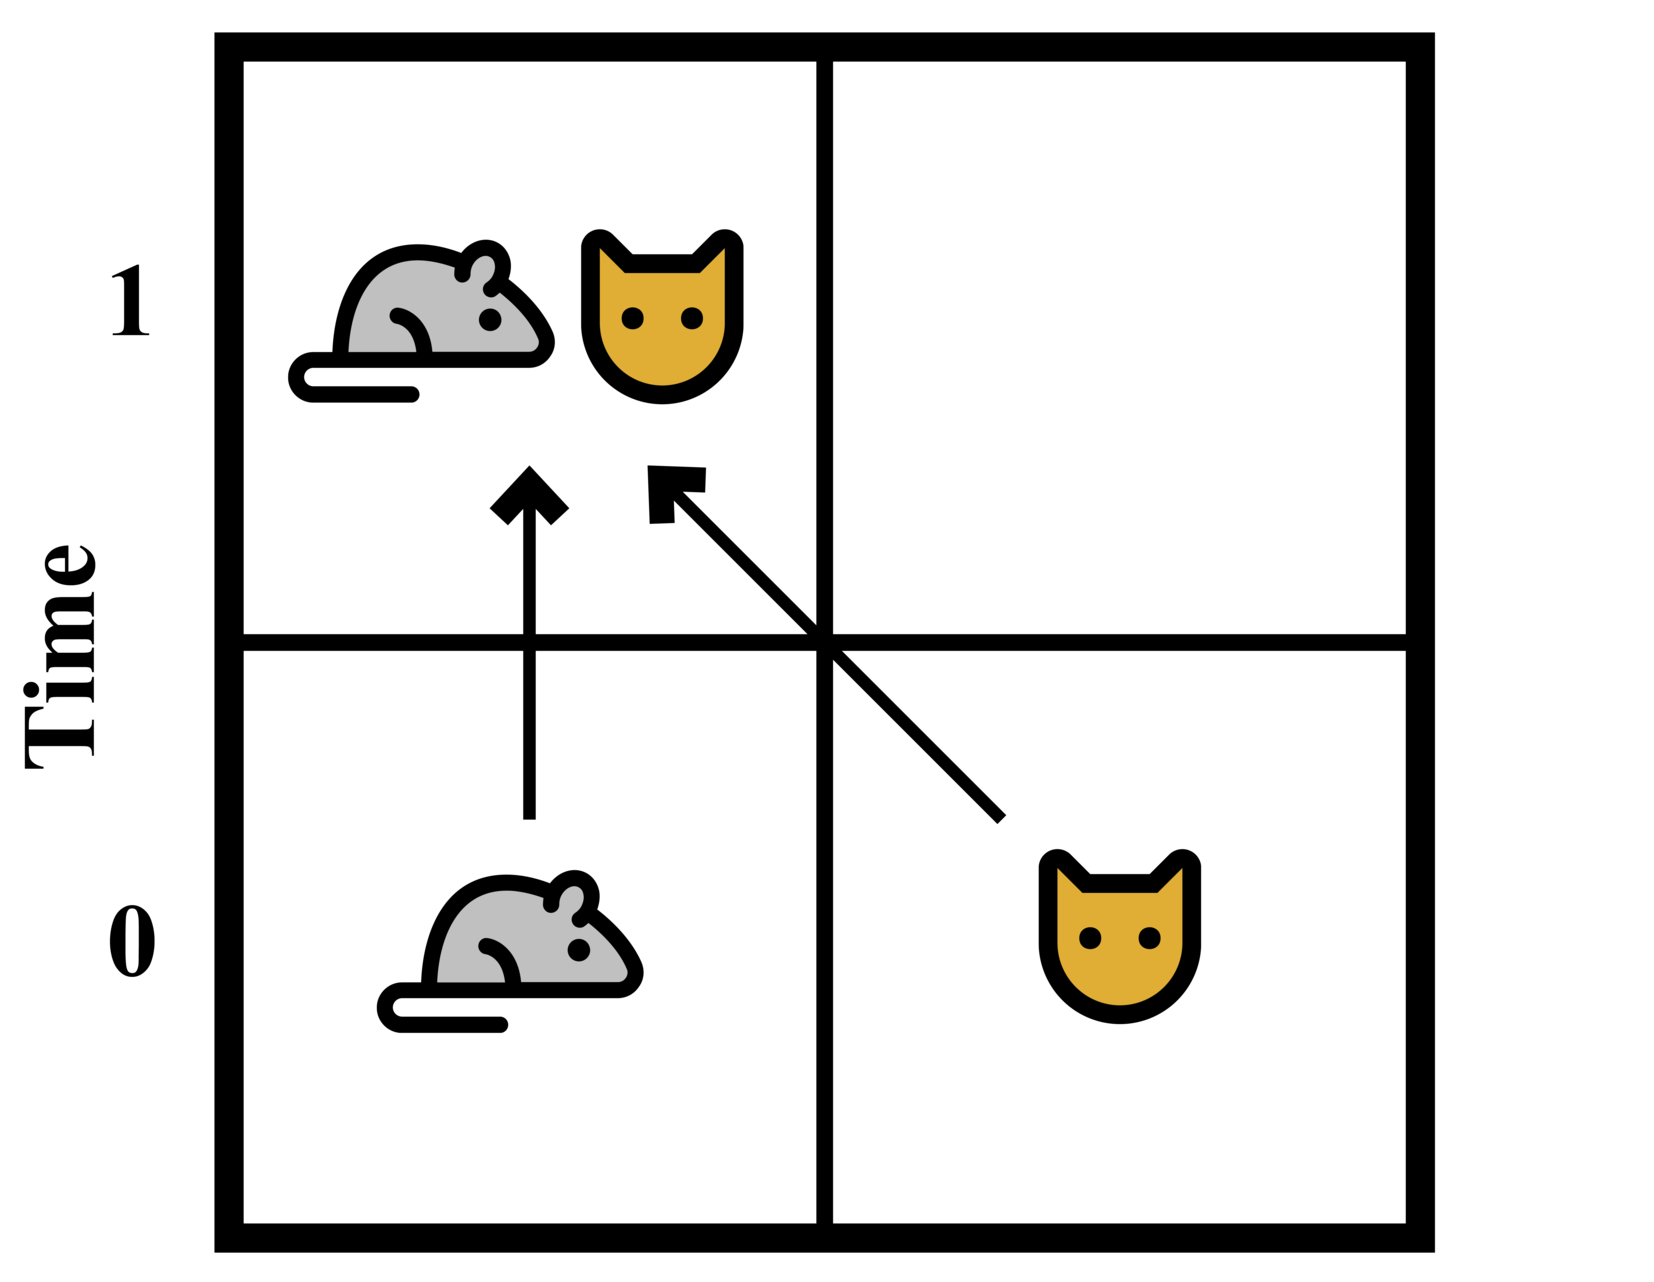
\includegraphics[scale=0.5]{figs/catMouseSm}
	}
	\caption{A simple cat and mouse model.\label{fig:AB-MCMC-1}}
\end{figure}


Let a model timestep consist of a matrix $E$ whose elements $e_{\psi a}$ are the number of agents in state $\psi$ that perform act $a$ in this timestep. For example, the timestep shown in Figure~\ref{fig:AB-MCMC-1} for the cat and mouse example would be
\[
E = \kbordermatrix{
	& A_0 & A_1 \\
	S_0 & 0 & 0 \\
	S_1 & 1 & 0 \\
	S_2 & 0  & 1 \\
	S_3 & 0 & 0 \\
}
\]
where all elements are zero except those representing agent $S_1$ (\textit{right cat}) performing action $A_0$ (\textit{move}) and agent $S_2$ (\textit{left mouse}) performing action $A_1$ (\textit{stay still}).

Let a model trajectory, $T$, be a tensor in $\mathbb{R}^N_{SA}$ that represents $N$ timesteps of a model with $S$ agent states and $A$ actions, so that $T^t_{\psi a}$ denotes the $(\psi, a)^{th}$ element of the $t^{th}$ timestep matrix.

A tensor must satisfy a number of constraints in order to be a valid trajectory of an ABM. Since the elements of a trajectory are counts of agents, they must be non-negative integers. We'll call this the \textit{non-negative integer constraint} and define the set of all non-negative integer tensors
\begin{equation}
\mathcal{I}^N_{SA} = \left\{ T \in \mathbb{R^N_{SA}}: \forall t,\psi, a: T^t_{\psi a} \ge 0, T^t_{\psi a} \in \mathbb{Z}\right\}
\label{nonNegativeInt}
\end{equation}

A trajectory must also be \textit{continuous} by which we mean that the number of agents in each state at the end of timestep $t-1$ must be the number of agents in each state at the beginning of timestep $t$\footnote{This does not mean that agents cannot leave or enter the system, only that if they do then that change must be defined as part of an action.}. We call this the \textit{continuity constraint} and define the set of continuous tensors, with respect to an action function $F$:
\begin{equation}
\mathcal{C}^N_{SA}(F) = \left\{T\in\mathbb{R}^N_{SA}:  \forall \left(  1 \le \bar t < N\right): F^{\psi a}_{\bar\phi} T^{\bar t-1}_{\psi a} = \mathbf{1}^aT^{\bar t}_{\bar\phi a}\right\}
\label{continuous}
\end{equation}
where $F^{\psi a}_\phi$ is the $\phi^{th}$ element of $F(\psi,a)$.


So, the set of valid trajectories, $\mathcal{T}^N_{SA}(F)$, is given by the set of tensors that satisfy \eqref{nonNegativeInt} and \eqref{continuous}.
\begin{equation}
\mathcal{T}^N_{SA}(F) = \mathcal{I}^N_{SA} \cap \mathcal{C}^N_{SA}(F)
\label{SetOfTrajectories}
\end{equation}


\subsection{The posterior}

Given a set of observations, $\Omega$, we'd like to sample from the posterior over the trajectories,
\[
P\left(T \middle| \Omega\right) \propto P(T)P\left(\Omega \middle| T\right)
\]
The prior over the trajectory can be composed from terms involving the agent timestep function, $\pi(\psi,\Psi^t,a)$, which gives the probability that a single agent will perform action $a$ given that it starts in state $\psi$ and is surrounded by agents $\Psi^t$. First consider all agents in state $\psi$ at the beginning of timestep $t$. Let $R\in\mathbb{R}_A$ be a vector whose elements $R_a$ are the number of these agents that perform act $a$ in timestep $t$. $R$ is just a multinomial distribution
\begin{equation}
P\left(R \mid \Psi^t, \psi\right) = 
\begin{cases}
\Psi^t_\psi!\prod_a \frac{\pi(\psi,\Psi^t,a)^{R_ a}}{R_a!} & \text{ if } R_a\mathbf{1}^a = \Psi^t_\psi \\
0 & \text{otherwise}
\end{cases}
\end{equation}
If we now let $P(\Psi^0)$ be the prior probability over the number of agents in each state at the beginning of the trajectory then the prior over trajectories can be written 
\begin{equation}
P(T) =
\begin{cases}
P(\Psi^0_{\bar\psi} = T^0_{\bar\psi c}\mathbf{1}^c)
\prod_{t, \psi}\left(T^t_{\psi b} \mathbf{1}^b \right)!
\prod_a \frac{\pi(\psi, T^{t}_{\bar\phi d}\mathbf{1}^d,a)^{T^{t}_{\psi a}}}{T^{t}_{\psi a}!} & \text{if } T \in \mathcal{T}^N_{SA}(F) \\
0 & \text{otherwise}\\
\end{cases}
\end{equation}

The likelihood can also be decomposed. Without loss of generality, we take $\Omega$ to consist of some number of observations that are independent of each other given the trajectory, so that $\Omega$ is a set of pairs $(\omega,v)$ that consist of a stochastic observation operator $\omega$ and an observed value $v$ (which may be a vector). We write $P(\omega(T)=v)$ to denote the probability of observation operator $\omega$ making observation $v$ on trajectory $T$. So
\[
P(\Omega|T) = \prod_{(\omega,v) \in \Omega} P(\omega(T)=v)
\]

The posterior can now be written as
\begin{equation}
P(T|\Omega) \propto 
\begin{cases}
\prod_{(\omega,v) \in \Omega,t, \psi, a}
P(\Psi^0_{\bar\psi} = T^0_{\bar\psi c}\mathbf{1}^c)
P\left(\omega(T)=v\right)
\left(T^t_{\psi b} \mathbf{1}^b \right)!
\frac{\pi(\psi, T^{t}_{\bar\phi d}\mathbf{1}^d,a)^{T^{t}_{\psi a}}}{T^{t}_{\psi a}!} & 
 \text{if } T \in \mathcal{T}^N_{SA}(F) \\
0 & \text{otherwise}\\
\end{cases}
\label{posterior}
\end{equation}

The problem we're interested in is how to sample from this distribution. In many practical applications, sampling is difficult because the posterior has zero probability for the vast majority of tensors (i.e. most tensors are not trajectories, contain an impossible action or are refuted by the observations). Even though we can generate trajectories that fit the prior by simply performing a forward execution of the model from an initial state drawn from the prior, if the observations refute the trajectory the probability falls to zero. It doesn't take many observations until the probability of randomly choosing a trajectory that fits the observations becomes very small indeed. So simple techniques such as rejection sampling, for example, are not practical. Techniques based on particle filtering may have more success but, for similar reasons, will likely soon reach a state containing a set of particles, none of which can be fit to the observations.

In the rest of this paper we'll show how to use the Metropolis-Hastings algorithm to generate samples from equation \eqref{posterior}. The challenge will be to create a proposal function which randomly generates a proposed next sample given the current one. A common strategy with Metropolis-Hastings is to generate a new sample by perturbing one or more elements of the previous sample at random. However, if we do this with a trajectory it's very unlikely that the perturbed tensor will be a trajectory that contains only possible actions and satisfies the observations. So, the proposed next sample would almost certainly be rejected and we'd probably end up stuck on the first sample until we grew old.

\section{Approximating the support of the posterior}
%##########################################

We solve this problem by first approximating the support of the posterior, $\supp(P(T|\Omega))$ (i.e. the set of trajectories that have non-zero probability).

From equation \eqref{posterior}
\begin{equation}
\begin{aligned}
\supp (P( T |\Omega)) = 
& \bigcap_{(\omega,v) \in \Omega,t, \psi, a} \mathcal{T}^N_{SA} \cap \\ 
&\supp(P(\Psi^0_{\bar\psi} = T^0_{\bar\psi c}\mathbf{1}^c)) \cap \\
& \supp\left(P\left(\omega(T)=v\right)\right) \cap \\
&\left( \supp\left(\pi(\psi,T^t_{\bar\phi b}\mathbf{1}^b,a)\right) \cup \left\{T:T^t_{\psi a} = 0\right\} \right)
\end{aligned}
\label{support}
\end{equation}
i.e. in order for $T$ to have non-zero posterior probability, it must be a trajectory of the ABM, it must have a start state that has non-zero prior probability, all the observation likelihoods must be non-zero and each element of $T$ must denote an agent action with non-zero probability.


\subsection{Convex $\mathbb{Z}$-polyhedra and $\mathbb{Z}$-distributions}
%################################################################
\label{BPoly}

Let a $\mathbb{Z}$-polyhedron be a set of tensors whose elements satisfy a set of linear constraints and belong to the set of integers: 
\[
\mathcal{P^N_{SA}} = \left\{ T\in\mathbb{\mathbb{Z}}^N_{SA} : L^{\bar i} \le  C^{\psi a\bar i}_t T^t_{\psi a} \le U^{\bar i} \right\}
\]
$C \in \mathbb{Z}^{SAI}_{N}$, $L \in \mathbb{Z}^I$ and $U \in \mathbb{Z}^I$ for some $I$. This is similar to the $\mathbb{Z}$-polyhedron described in \cite{quinton1996manipulating}).

From equation \ref{SetOfTrajectories} we can see immediately that $\mathcal{T}^N_{SA}$ is a  $\mathbb{Z}$-polyhedron. The supports of the prior, $P(\Psi^0)$, the observations, $P(\omega(T)=v)$, and the agent actions, $\pi(\psi,T^t\mathbf{1},a)$, can often be easily expressed as $\mathbb{Z}$-polyhedra. If this is not the case, each of the probability distributions can be expressed as computer programs. Once in this form, abstract interpretation tools\cite{cousot1977abstract} using the domain of convex polyhedra  \cite{cousot1978automatic}\cite{becchi2018efficient}\cite{fukuda2020polyhedral} can be used to construct a convex polyhedron that contains the support (note that it's fine to overestimate the support, i.e. include points that aren't in the support, but not to exclude points that are in the support. Abstract interpretation tools\cite{henry2012pagai}\cite{GN2021} are perfectly suited to this purpose). In addition, if the number of agents is very much smaller than the number of agent states (which is often the case with agent based models) then we may be willing to make the assumption that at any timestep there is at most one agent performing a given action from a given start state (i.e. $\forall \psi, a, t: T^{\psi a}_t \in \{0,1\}$). Under this assumption, which we'll call the \textit{Fermionic assumption} , the set of trajectories is a subset of the corners of the unit hypercube. Any such subset is a $\mathbb{Z}$-polyhedron.

So, if we let $\mathcal{P}^N_{SA}(f)$ be a $\mathbb{Z}$-polyhedron that over-approximates $\supp(f)$ on the integer points then from equation \eqref{support}
\begin{equation}
\begin{aligned}
\supp(P( T |\Omega)) \subseteq 
& \bigcap_{(\omega,v) \in \Omega,t,\psi, a} \mathcal{T}^N_{SA} \cap \\
& \mathcal{P}^N_{SA}(P(\Psi^0_{\bar\psi} = T^0_{\bar\psi c}\mathbf{1}^c)) \cap\\
&    \mathcal{P}^N_{SA}\left(P\left(\omega(T)=v\right)\right) \cap \\
& 
\left(\mathcal{P}^N_{SA}\left(\pi(\psi,T^t_{\bar\phi b}\mathbf{1}^b,a)\right)
\cup
\left\{T: T^t_{\psi a} = 0\right\}\right)
\\
\end{aligned}
\label{polyhedralSupport}
\end{equation}

The intersection of two $\mathcal{Z}$-polyhedra is easy to construct by just concatenating the constraints
\begin{multline}
\left\{ T\in\mathbb{\mathbb{Z}}^N_{SA} : L \le C^{\psi a \bar i}_{t} T^t_{\psi a} \le U \right\}
\cap \left\{ T\in\mathbb{\mathbb{Z}}^N_{SA} : L' \le D^{\psi a \bar i}_{t} T^t_{\psi a} \le U' \right\} \\
= \left\{ T\in\mathbb{\mathbb{Z}}^N_{SA} : {L \choose L'}  \le  {C^{\psi a\bar i}_t \choose D^{\psi a\bar j}_t} T^t_{\psi a} \le {U \choose U'} \right\}
\end{multline}
so the only difficulty is the union in the final term of \eqref{polyhedralSupport}. To transform this into an intersection we introduce an auxiliary variable $I^t_{\psi a}$ and use the identity
\begin{multline}
\left\{ T\in\mathbb{Z}^N_{SA} : L \le C^{\phi b\bar i}_{s} T^s_{\phi b} \le U \right\}
\cup
\left\{T: T^t_{\psi a} = 0\right\}
=\\
\left\{
T\in\mathbb{Z}^N_{SA}, I^t_{\psi a}\in\{0,1\}:\right.\\
-\infty \le C^{\phi b \bar i}_{s} T^s_{\phi b}
+
(\overline{B}-U)I^{t}_{\psi a}
\le \overline{B},\\
\underline{B} \le C^{\phi b \bar i}_{s} T^s_{\phi b}
+
(\underline{B}-L)I^{t}_{\psi a} \le \infty,\\
0 \le uI^t_{\psi a} - T^t_{\psi a},\\
\left. I^t_{\psi a} - T^t_{\psi a} \le 0
\right\}
\label{implication}
\end{multline}
where $u$ is the maximum value that any element of $T$ can take, the elements of $\overline{B}\in\mathbb{R}^I$ are defined as
\[
\overline{B}^i = \frac{u\sum_{s,\phi,b} \left( C^{\phi bi}_{s} + \left|C^{\phi bi}_{s}\right|\right)}{2}
\]
and the elements of $\underline{B}\in\mathbb{R}^I$ are defined as
\[
\underline{B}^i = \frac{u\sum_{s,\phi,b} \left(C^{\phi bi}_{s} - \left|C^{\phi bi}_{s}\right|\right)}{2}
\]

To see why this identity holds, note first that the constraints on $I^t_{\psi a}$ make it into an indicator variable that is 0 if $T^t_{\psi a}=0$ or 1 otherwise. When $I^t_{\psi a}=1$ the first set of constraints is equal to $C^{\phi b\bar i}_{s} T^s_{\phi b} \le U$ and the second is equal to $L \le C^{\phi b\bar i}_{s} T^s_{\phi b}$ so their intersection is $L \le  C^{\phi b\bar i}_{s} T^s_{\phi b} \le U$ as required, whereas when $I^t_{\psi a}=0$ we have the constraints $\underline{B} \le C^{\phi b\bar i}_{s} T^s_{\phi b} \le \overline{B}$. But $\underline{B}^i$ and $\overline{B}^i$ are lower and upper bounds on the value of $C^{\phi bi}_{s} T^s_{\phi b}$ so this is satisfied for all trajectories, as required.

There are two things worth noting here. Firstly if we make the Fermionic assumption then $I^t_{\psi a} = T^t_{\psi a}$ and the auxiliary indicator variables become unnecessary. Secondly, we must impose a finite value for $u$, the maximum value that elements of the trajectory can take. In practice, this is not a problem as we can give $u$ a value such that the probability of any trajectory of interest having any element larger than $u$ is small.

Using this transformation the support of the posterior can be reduced to a $\mathbb{Z}$-polyhedron

The idea of a $\mathbb{Z}$-polyhedron as the support for a probability distribution naturally leads to the idea of a $\mathbb{Z}$-distribution which is a discrete probability distribution defined over the members of a $\mathbb{Z}$-polyhedron. From the above, it can be seen that the posterior distribution of an ABM trajectory can be expressed as a $\mathbb{Z}$-distribution.

As an illustration, consider a two-timestep trajectory of the cat and mouse model described in section \ref{abmdef}. Suppose we flip a fair coin to decide whether each agent state is occupied or empty at $t=0$. Suppose also that we observe a cat in the left grid-square at time $t=1$. Our aim is to construct a $\mathbb{Z}$-polyhedron, $\mathcal{P}^2_{4\,2}(P(T|\Omega))$, that describes the support of the posterior.

Working through \eqref{polyhedralSupport} term by term, the $\mathcal{T}^2_{4\,2}$ term is just the continuity constraints in \eqref{continuous}, which are already in linear form so we're done. The second term is the support of the prior. This constrains each agent state at $t=0$ to be at most 1, which can be expressed as
\[
\left\{T:T^0_{\bar \psi 0} + T^0_{\bar\psi 1} \le \mathbf{1}_{\bar\psi}\right\}
\]

The third term is the support of the observation. Since we observe a cat in the left grid-square at time $t=1$ we need to add the constraint
\[
T^1_{0 0} + T^1_{0 1} = 1
\]
The final term is the constraint due to agent interactions. The impossible interactions are a mouse staying put when there is a cat on the same gridsquare or moving when there are no cats, which translates to the four cases
\begin{equation}
\begin{aligned}
\supp(\pi(2,T^t_{\bar\phi a}\mathbf{1}^a,0)) &= \left\{ T: -T^t_{0 0} - T^t_{0 1} \le -1 \right\}\\
\supp(\pi(3,T^t_{\bar\phi a}\mathbf{1}^a,0)) &= \left\{ T: -T^t_{1 0} - T^t_{1 1} \le -1 \right\}\\
\supp(\pi(2,T^t_{\bar\phi a}\mathbf{1}^a,1)) &= \left\{ T: T^t_{0 0} + T^t_{0 1} \le 0 \right\}\\
\supp(\pi(3,T^t_{\bar\phi a}\mathbf{1}^a,1)) &= \left\{ T: T^t_{1 0} + T^t_{1 1} \le 0 \right\}
\end{aligned}
\label{actionConstraints}
\end{equation}
for all t. If, for simplicity, we make the Fermionic assumption by adding the constraints
\[
\forall t,\psi,a: 0 \le T^t_{\psi a} \le 1
\]
then using the identity in \eqref{implication} to take the union of each constraint in \eqref{actionConstraints} with $\left\{T: T^t_{\psi a} = 0\right\}$ finally gives the four constraints
\[
\begin{aligned}
-T^t_{0 0} - T^t_{0 1} + T^t_{2 0} & \le 0\\
-T^t_{1 0} - T^t_{1 1} + T^t_{3 0} & \le 0\\
T^t_{0 0} + T^t_{0 1} + 2T^t_{2 1} & \le 2 \\
T^t_{1 0} + T^t_{1 1} + 2T^t_{3 1} & \le 2
\end{aligned}
\]
for each timestep $t=0$ and $t=1$ to describe the agent interactions.

Taken together, these constraints define a $\mathbb{Z}$-polyhedron that is the set of (Fermionic) trajectories for the cat and mouse ABM, and when combined with equation \eqref{posterior} defines $P(T|\Omega)$ as a $\mathbb{Z}$-distribution.

\section{Sampling from a $\mathbb{Z}$-distribution}
%#################################################

Now that we have shown how to express $P(T|\Omega)$ as a $\mathbb{Z}$-distribution, we now show how to construct a Markov process which will allow us to sample from a $\mathbb{Z}$-distribution.

To do this we need to define
\begin{itemize}
\item a set of Markov states, $\mathcal{M}$

\item a probability measure $P: \mathcal{M} \to \mathbb{R}$ which gives the probability of each Markov state (this need not be normalised, though, as we'll only ever be interested in probability ratios)

\item a stochastic proposal function $f:\mathcal{M} \to \mathcal{M}$ from which we can generate transitions to a new Markov state given the current Markov state

\item a mapping $E:\mathcal{M} \to \mathbb{R}^T_{SA}$ which maps Markov states to trajectories so we can recover the sample.
\end{itemize}

In order to be useable in the Metropolis-Hastings algorithm, the proposal function, $f$, must have the following properties:
\begin{itemize}
	\item For any two Markov states there should exist a set of transitions with non-zero probability which forms a path between those states.
	
	\item For any transition from state $S_a \to S_b$ with non-zero probability, the probability of the reverse transition from $S_b \to S_a$ should also be non-zero. This allows us to attain detailed balance in the Metropolis Hastings algorithm. The average ratio of forward and backward probabilities times the ratio of start and end state probabilities should be close to 1 to ensure that a reasonable proportion of proposals are accepted.
	
	\item Given a current Markov state, there should be computationally efficient ways of generating a proposal and calculating the acceptance probability. 
\end{itemize}


\subsection{The set of Markov states}
%#############################################

Given a $\mathbb{Z}$-polyhedron, we split the constraints into two sets: equalities (i.e. those whose lower and upper bound have the same value) and inequalities (i.e. those whose lower and upper bounds differ):
\begin{equation}
\mathcal{P} = \left\{T \in \mathbb{Z}^N_{SA}: L \le C^{\psi a\bar i}_t T^t_{\psi a} \le U \cap D^{\psi a \bar i}_t T^t_{\psi a} = E \right\}
\label{bPolySupport}
\end{equation}
Suppose there are $N_e$ equality constraints (i.e. $E$ is an $N_e$ dimensional vector) and we partition the elements of $T$ into `basic' and `non-basic' elements, so that there are exactly $N_e$ basic elements and $N\times S \times A - N_e$ non-basic elements.

Given such a partition we can define tensors $Q\in\mathbb{R}_{SAN_e}^{N}$ and $R\in\mathbb{R}_{SAJ}^{N}$, where $J=NSA - N_e$, that take `flattened' vectors of basic, $X\in\mathbb{R}^N_e$, and non-basic, $Y\in\mathbb{R}^J$, variables and project them into a trajectory tensor such that
\[
T^{t}_{\psi a} =  Q_{\psi ai}^{t} X^i + R_{ \psi  aj}^{t} Y^j
\]
If we now let
\[
B_i^k = D^{\psi ak}_{t}Q_{\psi a i}^{t}
\]
and
\[
N_j^k = D^{\psi ak}_{t}R_{\psi aj}^{t}
\]
then we can write the equality constraints as
\begin{equation}
B_i^kX^i + N_j^kY^j = E^k
\label{eqconstraints}
\end{equation}

Now, since there are $N_e$ basic variables and $N_e$ equality constraints, $B$ is square so if we choose the basic variables in order to ensure that $B$ has an inverse then
\begin{equation}
X^i = (B^{-1})^i_k(E^k + N_j^kY^j)
\label{basicvars}
\end{equation}
So, we define a Markov state to be an assignment to a non-basic variable vector $Y$ and map this to the trajectory using
\begin{equation}
T^t_{\psi a} =  Q_{\psi ai}^{t}(B^{-1})^i_k(E^k + N_j^kY^j) + R_{\psi aj}^{t } Y^j
\label{markovtotrajectorytensor}
\end{equation}
subject to
\[
0 \le Y_j \le u
\]
where $u$ is the upper limit on the occupancy of agent actions.

Equation \eqref{markovtotrajectorytensor} can be written as
\begin{equation}
T^t_{\psi a} =  K^t_{\psi a} + M^{t}_{\psi aj} Y^j
\label{markovtotrajectory}
\end{equation}
where
\[
K^t_{\psi a} = Q_{\psi ai}^{t} (B^{-1})^i_kE^k
\]
and
\[
M^{t}_{\psi aj} = Q_{\psi ai}^{t} (B^{-1})^i_kN_j^k + R_{\psi aj}^{t}
\]

\subsection{The probability of a Markov state}

Given a Markov state, $Y$, that satisfies $0 \le Y_j \le u$, the associated trajectory given by equation \eqref{markovtotrajectory} is guaranteed to satisfy all the equality constraints. However, there is no guarantee that the basic variables given by eq \eqref{basicvars} will be within their bounds or that the inequality constraints will be satisfied. To deal with this we introduce the concept of \textit{infeasibility} which is a measure of how far a Markov state is from being feasible.

Given the inequality constraints of the $\mathbb{Z}$-distribution (including the upper limits of the basic variables themselves)
\[
L^i \le C^{\psi ai}_{t} T^t_{\psi a} \le U^i
\]
using \eqref{markovtotrajectory} this can be written as
\begin{equation}
L^i \le J^i + Q_j^i Y^j \le U^i
\label{ineqconstraints}
\end{equation}
where
\[
J^i = C^{\psi ai}_{t} K^t_{\psi a}
\]
and
\[
Q_j^i = C^{\psi ai}_{t}M^{t}_{\psi aj}
\]

let the infeasibility of the $i^{th}$ constraint, $\iota(Y)_i$, be defined to be equal to 0 if the constraint is satisfied or equal to the distance to the nearest bound otherwise
\[
\iota(Y)_i =
\begin{cases}
L^i- J^i - Q_j^iY^j & \text{if }J^i + Q_j^iY^j<L^i\\
J^i + Q_j^iY^j-U^i & \text{if }J^i + Q_j^iY^j>U^i\\
0 & \text{otherwise}
\end{cases}
\]
and let the total infeasibility be the sum of infeasibilities of all constraints
\[
\iota(Y) = \sum_i \iota(Y)_i
\]
So, each Markov state is associated with a total infeasibility with respect to the inequalities of the $\mathbb{Z}$-distribution. 

If the infeasibility is zero, then all the constraints are satisfied and the probability is defined by the $\mathbb{Z}$-distribution
\[
P(Y) = P(K^t_{\psi a} + M^{t}_{\psi aj}Y^j)
\]

If the infeasibility is not zero, then the probability is defined in the following way. Given an upper bound on the trajectory's elements, $u$, we define the \textit{clamped} trajectory
\[
\overline{\underline{T^t_{\psi a}}} = 
\begin{cases}
0 & T^t_{\psi a}<0\\
u & T^t_{\psi a}>u\\
T^t_{\psi a} & \text{otherwise}
\end{cases}
\]

Furthermore, let $H_t^{\psi a}$ be a log-linear approximation to the target $\mathbb{Z}$-distribution so that for feasible trajectories
\[
H_t^{\psi a}T^t_{\psi a} \approx \log(P(T))
\]
For infeasible trajectories, we define the probability, $P_\iota$, as
\begin{equation}
\log(P_\iota(Y)) = \sum_{t \psi a} H_t^{\psi a}\overline{\underline{K^t_{\psi a}+M^{t}_{\psi aj}Y^j}} + \kappa\iota(Y)
\label{loglinprob}
\end{equation}
where $\kappa < 0$ is a tunable parameter.

The probability of a Markov state, $Y$, is now given by
\begin{equation}
P(Y) =
\begin{cases}
P(Y) & \text{if } \iota(Y) = 0\\
P_\iota(Y) & \text{if } \iota(Y) > 0\\
\end{cases}
\end{equation}

This means that infeasible states have non-zero probability, so the Markov chain will pass through some infeasible states.  However, if we just ignore these and only take samples from feasible states then we end up with samples of the target $\mathbb{Z}$-distribution. Allowing the Markov chain to pass through infeasible states has the advantage of ensuring that there exists a path between any two feasible states and improves mixing. The disadvantage is the computational cost of moving through infeasible states that don't generate useful samples.

The infeasible Markov states are distributed as a Boltzmann distribution with a ``temperature'' of $\frac{-1}{\kappa}$.  It has been shown that thermodynamic systems of this type are able to solve large integer optimisation problems \cite{kirkpatrick1983optimization}. In our case, we don't need to change the temperature during the sampling process, but we do need to choose a value for $\kappa$. Higher temperatures will increase mixing in the Markov chain, but will also increase the proportion of time spent in infeasible states so we need to find a temperature that is high enough to ensure good mixing of the chain but low enough to ensure a reasonable proportion of samples are feasible. We have found that a good rule of thumb is to set the temperature so that 50\% of the states in a chain are infeasible.

\subsection{Transitions between Markov states}

Given a Markov state, we can transition to another state by choosing an element of  $Y$ and perturbing it by $\pm 1$ (or, if the element is on one of its bounds then to perturb it away from the bound in the feasible direction. In the case of Fermionic trajectories, the elements of $Y$ are always on their bounds so there is always exactly one perturbation per element: a swap to the other bound). This defines the set of transitions between Markov states. Let the set of all Markov states reachable from state $Y$ be denoted by $\mathcal{D}(Y)$. 

\subsubsection{The probability of transitions}

The probability of a transitions from $Y$ to $Y'$ is defined to be
\[
P(Y \to Y') = \frac{\min\left(1, \frac{P_\iota(Y')}{P_\iota(Y)}\right)}{S(Y)} 
\]
where $P_\iota$ is the log-linear probability defined in \eqref{loglinprob} and
\[
S(Y) = \sum_{Y'\in \mathcal{D}(Y)}\min\left(1, \frac{P_\iota(Y')}{P_\iota(Y)}\right)
\]
Note that this is irrespective of whether $Y$ or $Y'$ are feasible.

Given this, the Metropolis-Hastings acceptance probability is
\[
\alpha = \frac{P(T')P(Y' \to Y)}{P(T)P(Y \to Y')} = 
\frac{P_\iota(Y)}{P(Y)} \frac{P(Y')}{P_\iota(Y')}  \frac{S(Y)}{S(Y')}
\]

When $Y$ is infeasible $\frac{P_\iota(Y)}{P(Y)} = 1$. When $Y$ is feasible $P_\iota(Y)$ approximates $P(Y)$ so their ratio should be close to 1. Finally, $S(Y)$ will not change very much between transitions so the ratio $ \frac{S(Y)}{S(Y')}$ should also be close to 1 meaning that the acceptance probability should also be close to 1.

\subsection{Choosing a basis}

TODO: need to start with auxiliary variables for equality constraints...or factorize out columns one at a time starting with (X|Y) as a flattening of T and all variables considered non-basic and the factorized part as the 'proper' basic variables (i.e. same as with aux variables but they're implicit).

The definition of the Markov chain depends on a partition of the trajectory into basic and non-basic elements. We now describe how such a partition is chosen. 

If we let
\[
F^j_i = C^{\psi a j}_tQ^t_{\psi a i}
\]
and
\[
G^j_i = C^{\psi aj}_tR^t{\psi a i}
\]
then we can combine the equality constraints \eqref{eqconstraints} and inequality constraints \eqref{ineqconstraints}
\[
{0 \choose L} \le
\begin{pmatrix}
B & N\\
F & G
\end{pmatrix}
{X \choose Y} + {-E \choose J} \le {0 \choose U}
\]
then
\[
{0 \choose L} \le
\begin{pmatrix}
I & B^{-1}N\\
F & G
\end{pmatrix}
{X \choose Y} + {-B^{-1}E \choose J} \le {0 \choose U}
\]
and
\[
{0 \choose L} \le
\begin{pmatrix}
I & B^{-1}N\\
0 & G-FB^{-1}N
\end{pmatrix}
{X \choose Y} + {-B^{-1}E \choose J + FB^{-1}E} \le {0 \choose U}
\]


where $I$ is the identity matrix.

If we let $S_{ij}$ be the permutation matrix such that
\[
{X'\choose Y'} = S_{ij}{X\choose Y}
\]
has the effect of swapping the $i^{th}$ element of $X$ with the $j^{th}$ element of $Y$ then we have
\[
\begin{pmatrix}
I & N\\
CQ & CR
\end{pmatrix}
S^{-1}_{ij}{X' \choose Y'} = b
\]
(note that $S^{-1}_{ij} = S_{ij}$).

If we now pre-multiply this with the matrix 
\[
B_{ij}^{-1} =  
\begin{pmatrix}
1 &  & -\frac{N_{0j}}{N_{ij}} & & \\
& \ddots & \vdots & &\\
& & \frac{1}{N_{ij}} & &\\
& & \vdots & \ddots &\\
& & -\frac{N_{nj}}{N_{ij}} & &1\\
\end{pmatrix}
\]
it can be shown \cite{maros2002computational} that
\begin{equation}
B_{ij}^{-1}(I|N)S^{-1}_{ij} = (B_{ij}^{-1}|B_{ij}^{-1}N)S^{-1}_{ij} = (I|N')
\label{Ntransform}
\end{equation}
and so
\begin{equation}
B_{ij}^{-1}(I|N)S^{-1}_{ij}{X'_B \choose X'_N} = B_{ij}^{-1}b  = (I|N'){X'_B \choose X'_N} = b'
\end{equation}
Now, if we choose an $i$ and $j$ such that $N_{ij} = \pm 1$, then all elements of $B^{-1}_{ij}$ are integer and so all elements of $N'$ are also integer, as are the elements of $b'$. This ensures that if $X_N\in\mathbb{Z}^J$ then $X_B\in\mathbb{Z}^I$ and $X\in\mathbb{Z}^K$ as required.

So if we let
\[
Q' = QS^{-1}_{ij}
\]
we can express the original $\mathbb{Z}$-polyhedron in the equivalent form
\begin{equation}
\mathcal{P} = \left\{X\in\mathbb{Z}^K: X = Q'{X'_B\choose X'_N}, X'_B = b'-N'X'_N, S_{ij}L \le {X'_B \choose X'_N} \le S_{ij}U, X'_B \in \mathbb{Z}^I, X'_N \in \mathbb{Z}^J \right\}
\end{equation}

It is easy to see that this transformation defines an equivalence set so that, given a reference representation of a $\mathbb{Z}$-polyhedron, $\mathbb{Z}(Q,N,b,L,U)$, we can define the set of all equivalent ``pivot states'' $\mathcal{S}(Q,N,b,L,U)$.


\subsection{An efficient proposal algorithm}

We next provide an efficient algorithm to choose a proposal with the correct probability from the set of transitions given the current Markov state.

TODO: Finish this


\section{Results}

\section{Further work}
\subsection{Abstract interpretation using convex polyhedra}

In many cases a $\mathcal{B}$-polyhedron of the set of Fermionic trajectories in the support of the prior, observations and timestep of an agent can easily be constructed by hand in the form of a set of linear inequalities. In some cases, however, it may be less obvious how to construct this. In this case the linear inequalities can be constructed automatically from a computer program that calculates the function whose support we're trying to find.





The first two terms in equation \eqref{support} consists of the supports of computer programs whose inputs are ABM trajectories and whose outputs are given, i.e. the set of trajectories that, when passed to a computer program, would produce a given output.

Calculating the support of a computer program for a given output is, in full generality, NP-complete\footnote{Consider, for example, a program that accepts an assignment of variables to truth values, and returns true if that assignment satisfies a Boolean formula. Deciding whether the support of this program, given that it returns true, is empty or not is equivalent to solving the Boolean satisfiability problem, which is known to be NP-complete\cite{cook1971complexity}} but it is possible to use a technique known as \textit{abstract interpretation}\cite{cousot1977abstract} to efficiently calculate a superset of the support. So, given a computer program $\rho$, we can calculate a set $\mathcal{P}(\rho, v)$ such that
\[
\supp(P(\rho(.)=y)) \subset \mathcal{P}(\rho, v)
\]
Tools to perform abstract interpretation already exist (e.g. PAGAI\cite{henry2012pagai}) and are used widely in applications such as the verification of safety critical systems\cite{blanchet2003static} and in practice $\mathcal{P}(\rho, v)$ is often reasonably tight (i.e. most members of $\mathcal{P}(\rho, v)$ are in $\supp(P(\rho(.)=y))$). For our application we choose to express $\mathcal{P}(\rho, v)$ in terms of a set of linear inequalities on $\rho$'s inputs, this corresponds to the abstract domain of convex polyhedra\cite{cousot1978automatic}\cite{becchi2018efficient}. Calls to the random number generator can be dealt with in the abstract domain by generating a new variable, $r$, that satisfies $0 \le r < 1$ for each call to \texttt{Random()}. These can either be left in as ``auxiliary'' variables in the same way as slack variables, or removed as soon as the variable goes out of scope by finding the convex hull of the projection into a lower dimensional space (this can be done using the double description method\cite{motzkin1953double}).


Constraining our proposal function to members of the superset in equation \eqref{linearSupport} instead of the true support won't affect the stationary distribution of the Markov Chain. If the proposal function happens to return a trajectory that isn't in $\supp(P(\rho(.)=y))$ then it will just be rejected. This is fine as long as we generate acceptable proposals at a reasonable rate.

\section{Conclusion}

\section{Notes}

Why does convergence scale so badly with number of timesteps? Probably because as the number of non-zero elements per col/row increases, so does the average energy change in a feasible to infeasible transition, so we must increase the temperature to get the same amount of mixing. This results in a lot more time spent in infeasible space. 

\subsection{Fermionic Trajectories}

In the following we will consider only \textit{Fermionic trajectories}, which we define to be any trajectory whose elements are all either 0 or 1. i.e. a Fermionic trajectory must not only satisfy the constraints in \eqref{nonNegativeInt} and \eqref{continuous} but must also satisfy the \textit{Fermionic constraints}
\begin{equation}
\mathcal{B}^N_{SA} = \left\{T\in\mathbb{R}^N_{SA} : \forall t,\psi,a: T^t_{\psi a} \in \left\{ 0,1 \right\}\right\}
\label{fermionic}
\end{equation}
This can be interpreted as meaning that no two agents in the same state at the same time can perform the same action. Notice that the Fermionic constraints imply the non-negative integer constraints, so the set of Fermionic trajectories, $\mathcal{F}^N_{SA}$, is the set of tensors that satisfy \eqref{fermionic} and \eqref{continuous}.
\begin{equation}
\mathcal{F}^N_{SA}(F) = \mathcal{B}^N_{SA} \cap \mathcal{C}^N_{SA}(F)
\end{equation}

If we now condition the posterior on $T \in \mathcal{B}^N_{SA}$ then the support of the posterior becomes
\begin{equation}
supp(P(T|\Omega, T\in\mathcal{B}^N_{SA})) = \mathcal{B}^N_{SA} \cap supp(P(T|\Omega))
\label{fermionicSupport1}
\end{equation}

In practice, the number of agents in an ABM is usually much smaller than the number of agent states, so it is overwhelmingly likely that a sample from the posterior will be Fermionic, and so intersection with $\mathcal{B}^N_{SA}$ will often have very little effect on the posterior. However, section ** describes how to extend the algorithm to apply to non-Fermionic trajectories when the Fermionic constraints are not acceptable.

\begin{theorem}
	For any set $\mathcal{X}$ there exists a convex polyhedron $P$ such that
	\[
	\mathcal{B}^N_{SA} \cap \mathcal{X} = \mathcal{B}^N_{SA} \cap \mathcal{P}
	\]
\end{theorem}
\begin{proof}
	Let $\mathcal{Y} = \mathcal{B}^N_{SA} \cap \mathcal{X}$ and let $\mathcal{P}$ be the convex hull of $\mathcal{Y}$. Clearly if a tensor $T\in \mathcal{Y}$ then $T\in \mathcal{B}^N_{SA} \cap \mathcal{P}$. To show the converse, suppose there is a member $T' \in \mathcal{B}^N_{SA} \cap \mathcal{P}$. Since $T'\in \mathcal{P}$ then there must be a convex combination of points in $\mathcal{Y}$ that equals $T'$. Call those points $\mathcal{Z}$. However, since $T' \in \mathcal{B}^N_{SA}$ and $\mathcal{Z}\subset \mathcal{B}^N_{SA}$ and no member of $\mathcal{B}^N_{SA}$ is a convex combination of any other member then $T'$ must be a member of $\mathcal{Z}$ and so $T'\in \mathcal{Y}$. So $\mathcal{B}^N_{SA} \cap \mathcal{X} = \mathcal{B}^N_{SA} \cap \mathcal{P}$. 
\end{proof}



%\bibliographystyle{unsrtnat}
%\bibliographystyle{apalike} 
\bibliographystyle{apacite}
\bibliography{references}

\end{document}
